\chapter{Data Processing} 
\label{chap:chap5}
This chapter describes the necessary steps to convert data between each of the levels described in the processing flowchart. Source code snippets are provided in Python.
\section{Overview}
The IDEX data processing pipeline takes the data packets described above, an xml XTCE definition/decommutation table (\ref{xtce}), the instrument ground calibration curve, the spacecraft thruster data, and ephemerides data as inputs. Each data product and its corresponding inputs/outputs is described in Figure \ref{fig:flow}.

\begin{figure}[H]
    \centering
                                                                                                                                                                                                                             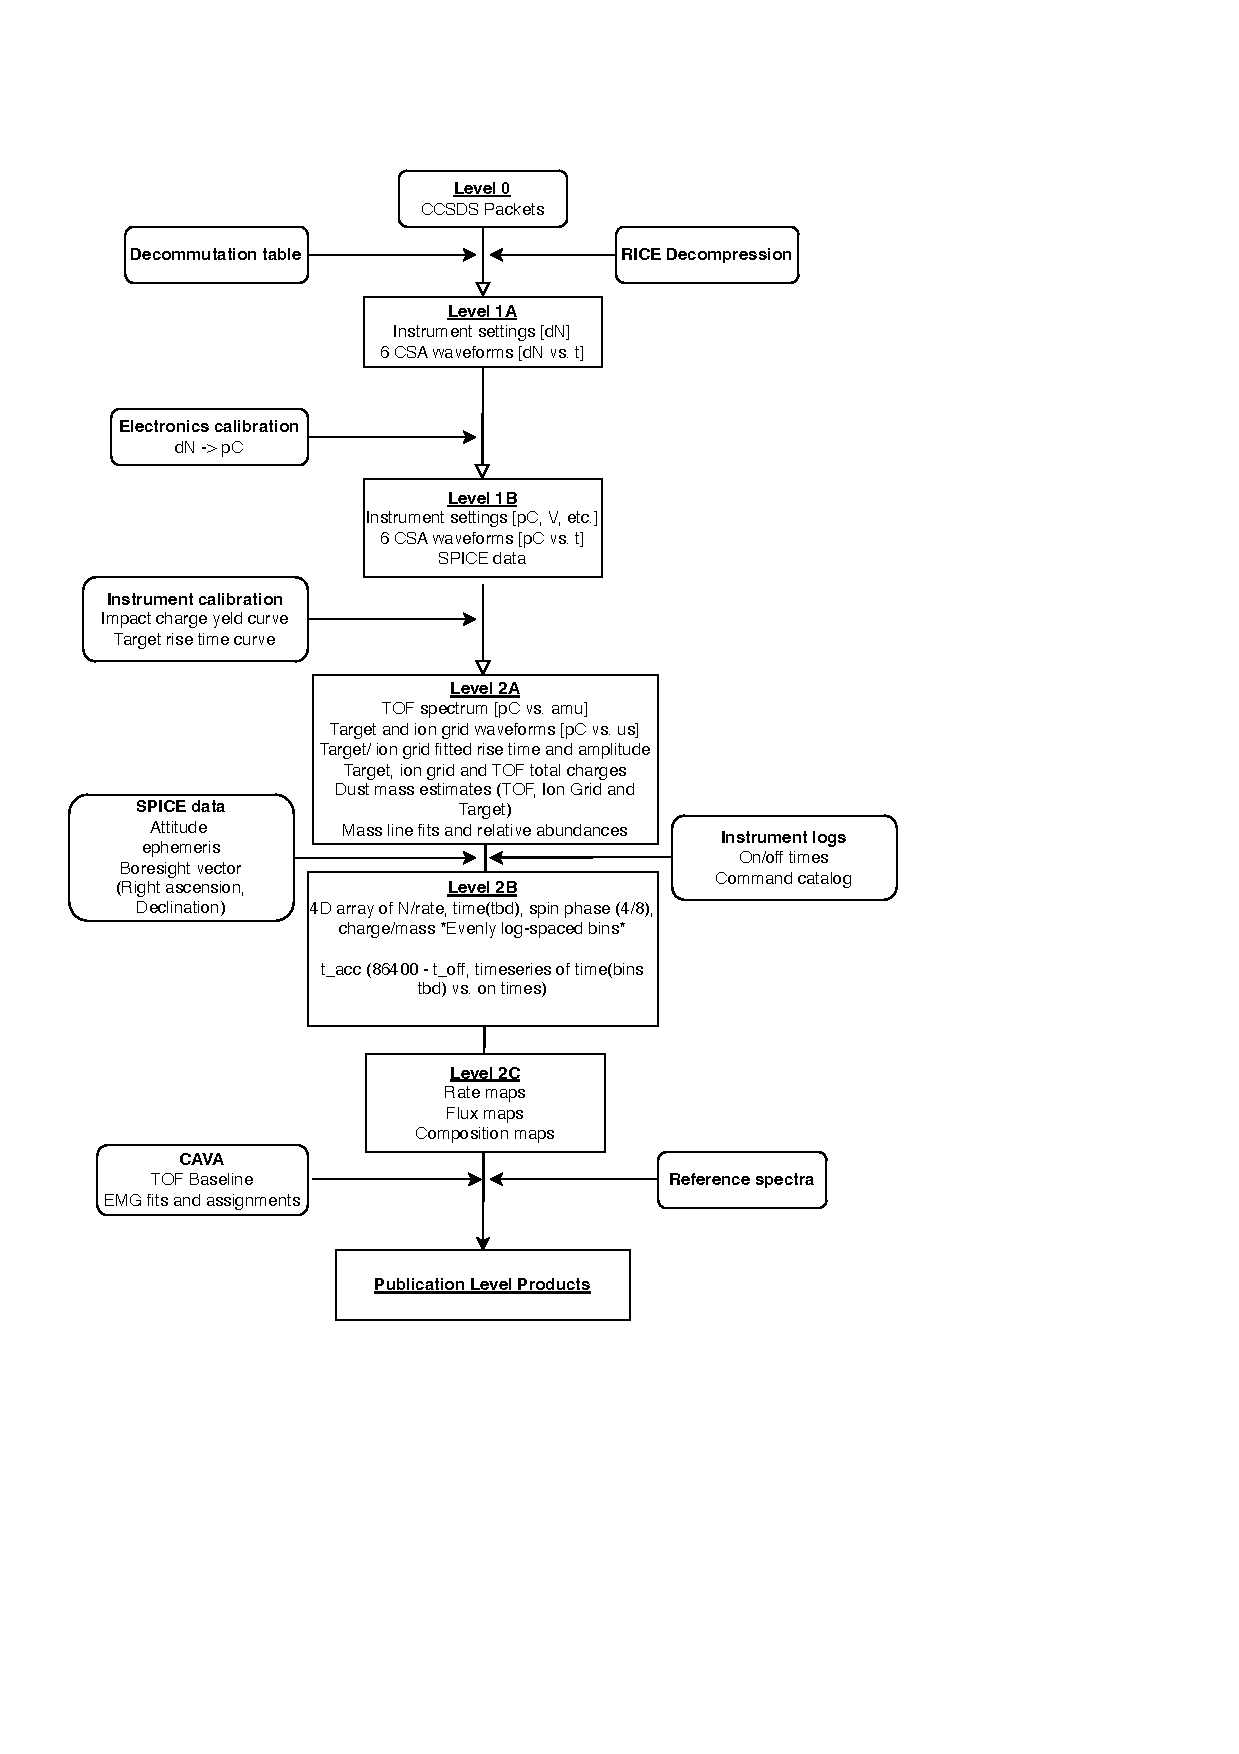
\includegraphics[width=.7\linewidth]{images/PipelineFlow_Updated.key.drawio.pdf}
    \caption{The IDEX science data pipeline processing flowchart. Data products are given in the center, with the necessary auxiliary inputs on the sides.}
    \label{fig:flow}
\end{figure}

\section{Data Volume Expectancy}

The estimates for the expected IDEX instrument science data volume are derived from simulations of known IDP and ISD populations. Figure \ref{fig:isdpop} depicts counts for ISD (red/blue) and IDP (black) particles expected to be measured by IDEX during the mission.

\begin{figure}[H]
    \centering
    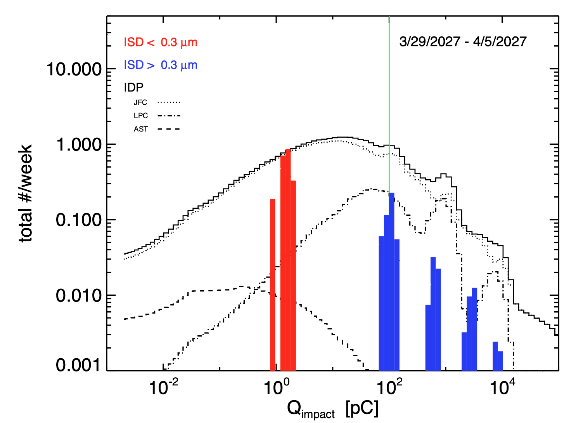
\includegraphics[width=.7\linewidth]{images/IDPISD.png}
    \caption{Expectations for IDEX's ISD and IDP measurements during the mission. Note that although this is just shown for 6 days in 2027, these simulations have been carried out for all of the prime and extended IMAP mission.}
    \label{fig:isdpop}
\end{figure}

From this simulation, IDEX is expected to measure 16 events per day on average. Using these estimates in conjunction with the bitmap in Figure \ref{fig:headbit}, we can estimate the weekly data volume expectancy for IDEX during the mission. This has been carried out for each of the science data product levels, as depicted in table \ref{fig:vol}.

\begin{table}[H]
    \centering
    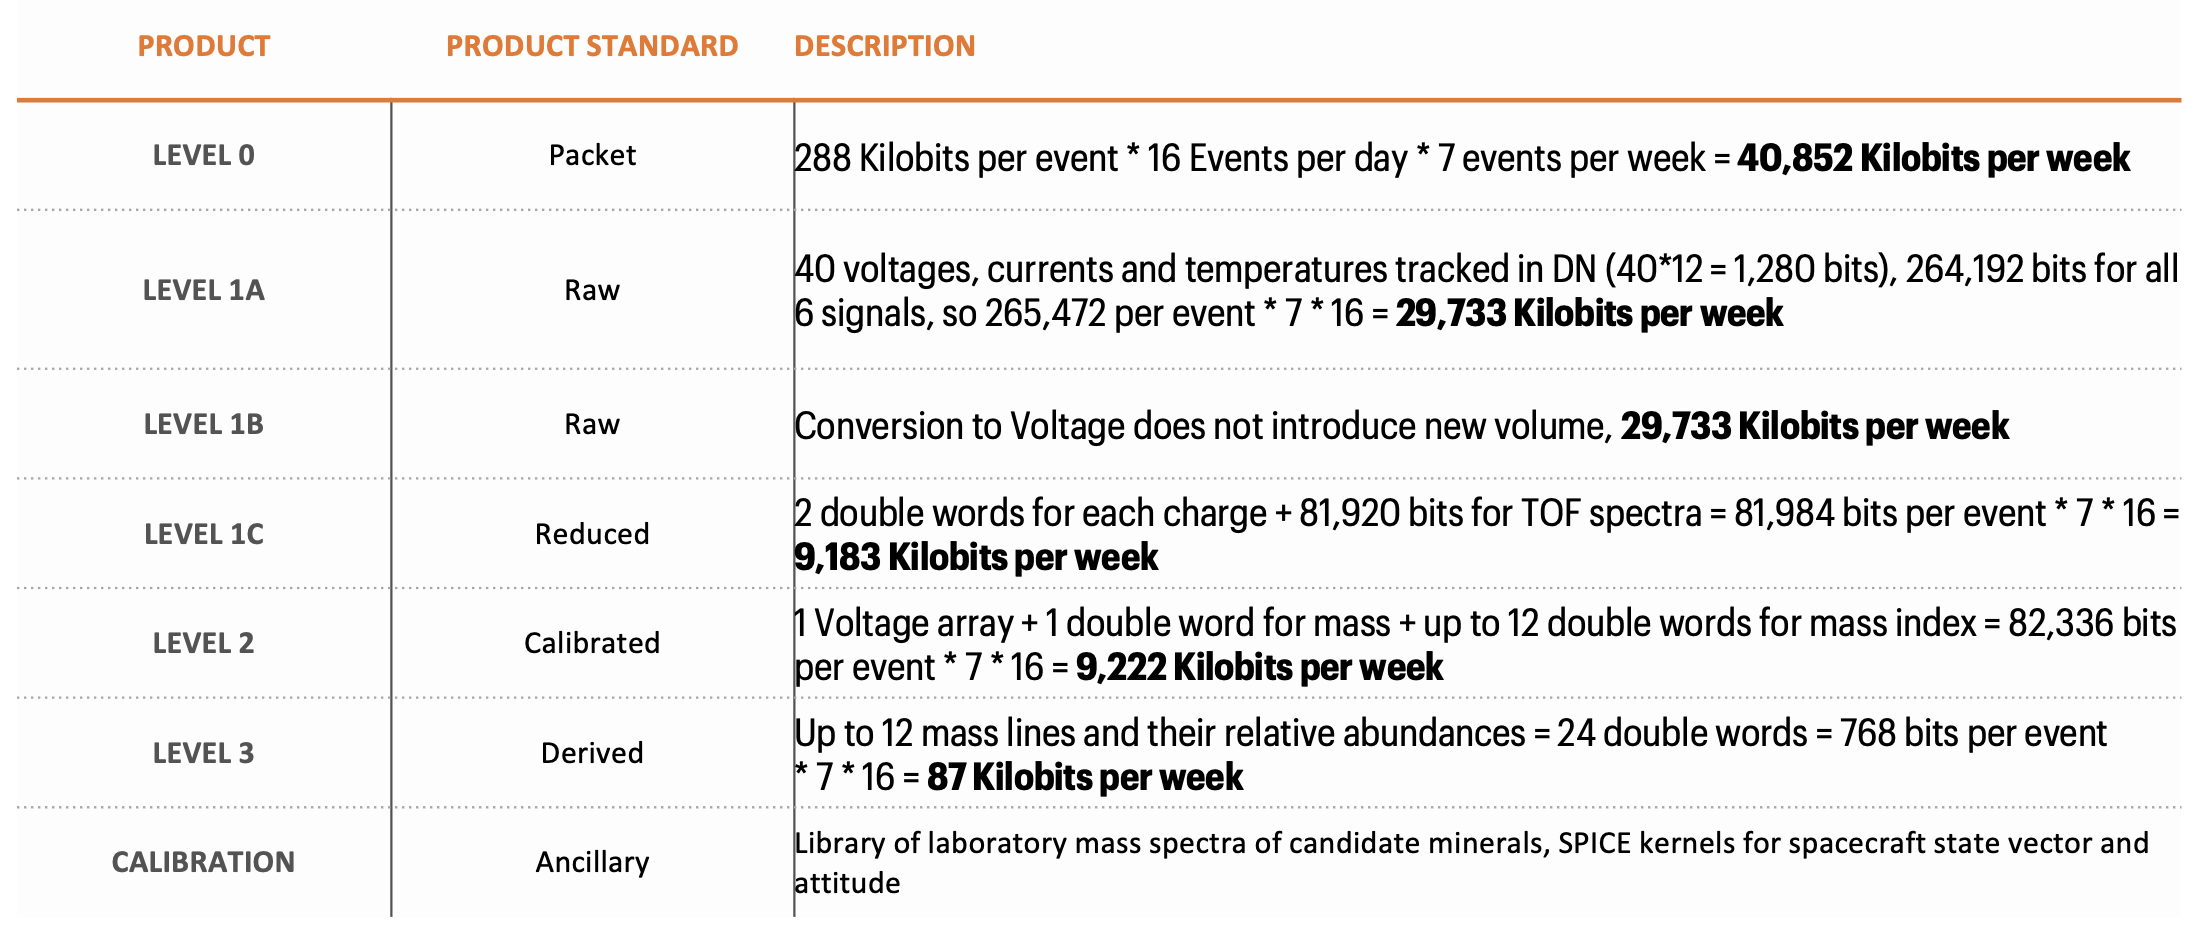
\includegraphics[width=\linewidth]{images/DataVolume.png}
    \caption{Expectations for IDEX's weekly data volume throughout the mission, organized by data product level.}
    \label{fig:vol}
\end{table}


\section{Heritage Data Processing}
IDEX has a high-level of heritage from the SUrface Dust Analyzer (SUDA) onboard the upcoming flagship \textit{Europa Clipper} mission. SUDA is nearly identical but has instead been optimized for flybys and detections of organic molecules for a limited impact velocity range of around 4 km/s.  The XTCE definition is the same for both instruments (see appendix \ref{xtce}), but the interpretation of the waveforms differs, along with voltage/temperature conversions.

Like IDEX, SUDA Event data is composed of seven distinct parts:
\begin{enumerate}
\item	Time of Flight (TOF) waveform data on the high-gain (HG) channel, sampled at 250 megasamples per second (Msps) with 10 bit resolution
\item	TOF waveform data on the mid-gain (MG) channel, sampled at 250 Msps with 10 bit resolution
\item	TOF waveform data on the low-gain (LG) channel, sampled at 250 Msps with 10 bit resolution
\item	Velocity (Qv) grid charge sensitive amplifier (CSA) waveform data, sampled at 3.75 Msps with 12 bit resolution
\item	Ion (Qi) grid CSA waveform data, sampled at 3.75 Msps with 12 bit resolution
\item	Target (Qt) CSA waveform data, sampled at 3.75 Msps with 12 bit resolution
\item	FPGA Pre-pended metadata header containing IDEX’s configuration and status at the time of the trigger, recorded by the FPGA
\end{enumerate}

The velocity grid CSA takes the place of IDEX's second target gain stage. Otherwise, the names, sampling rates, and bit resolutions are all identical. SUDA leverages the use of the SWIFT language-based SPECTRUM software, developed in-house at LASP. To avoid this Mac OS dependency, the IDEX pipeline has been constructed exclusively in Python 3.8.
\section{Level 0 to Level 1A Processing}
\subsection{Decommutation}
Packet decommutation relies on the \textbf{LASP packets} library, available on the \href{https://bitbucket.lasp.colorado.edu/projects/SDS/repos/lasp_packets/browse}{LASP Bitbucket (LASP VPN access required)}. The \textbf{LASP packets} software hinges on the \textbf{generator} method of the \textbf{Parsing.PacketParser} module for reading CCSDS packets (please see appendix \ref{lasppackets} for Python source code).

The packet data is read in using Python's \textbf{bitstring} library to reduce memory usage. Each packet is associated with a "flattened sequence container" from the XTCE definition. To do this, first, the length of the packet is taken from the CCSDS header:

\begin{minted}[breaklines, xleftmargin=20pt]{python}
specified_packet_data_length = self._total_packet_bits_from_pkt_len(header['PKT_LEN'].raw_value)
\end{minted}

Next, the type of packet as provided by the CCSDS header is cross-referenced with the XTCE definition to find a matching APID, VERSION, and TYPE. If there is a match, the code parses the packet according to the XTCE definition. If there is no match, it will attempt to generally parse it using the length of the packet. The source for this is shown below.

\begin{minted}[breaklines, xleftmargin=20pt]{python}
try:
                if isinstance(self.packet_definition, xtcedef.XtcePacketDefinition):
                    packet = self.parse_packet(binary_data,
                                               self.packet_definition.named_containers,
                                               root_container_name=root_container_name,
                                               word_size=self.word_size)
                else:
                    packet_def_name, parameter_list = self._determine_packet_by_restrictions(header)
                    packet = self.legacy_parse_packet(binary_data, parameter_list, word_size=self.word_size)

\end{minted}

This process is repeated until we have parsed each of the packets in the dataset.

\subsection{Science Data}
Once the data has been depacketized, the \textbf{SCI0TYPE} field designates what data is contained in each packet. Per the table in \ref{wavepack}, the possible values of \textbf{SCI0TYPE} include:
\begin{mdframed}[backgroundcolor=backcolour]{
 {\bf 1} = FPGA pre-pended metadata header \\
 {\bf 2} = TOF HG \\
 {\bf 4} = TOF LG \\
 {\bf 8} = TOF MG \\
 {\bf 10} = Target LG ($Q_T$) CSA \\
 {\bf 20} = Target HG ($Q_T$) CSA \\
 {\bf 40} = Ion grid ($Q_I$) CSA \\
} \end{mdframed}

By reading in the \textbf{SCI0TYPE} field, the appropriate ADC sampling rate (and therefore bit pattern) is determined.
\newpage 
The waveform data must be read in a pattern specific to high or low sampling rate ADCs in the schema outline below:

\begin{mdframed}[backgroundcolor=backcolour]{
\large For \textbf{high sampling rate (TOF) data (10-bit samples)}, handle the raw data as 32-bit units like this (most significant bit first):\newline 
\normalsize \\
  {\bf 2 bits} = Padding set to zeros, ignore this \\
  {\bf 10 bits} = oldest sample \\
  {\bf 10 bits} = next sample \\
  {\bf 10 bits} = next (newest) sample \\ 
\newline
\noindent \large For the remaining \textbf{low sampling rate data (12-bit samples)}, handle the raw data as 32-bit units like this (most significant bit first):\newline 
 \normalsize \\
  {\bf 8 bits} = Padding set to zeros, ignore this \\
  {\bf 12 bits} = oldest sample \\
  {\bf 12 bits} = next (newest) sample \\
} \end{mdframed}

Once this schema has been used for the waveform data, all the science event data has been read in and stored. The example Python script below will read in an IDEX raw binary data file, plot each of the event waveforms, and write all of the data to an easily accessible HDF5 file. Plots are saved to a \textit{/Plots/} directory in the same directory as the script, and the HDF5 files are written to the \textit{/HDF5/} directory.


It has been updated to be used as a command line tool, so we may use:
\begin{minted}[breaklines]{python}
python idex_packet.py --file filename
\end{minted}
Where $filename$ must be replaced with the name of the packet file, and $python$ must be an alias for a python installation. The $--file$ can be substituted for $-f$.

\subsection{Metadata translation and timing validation}
The HDF5 writer now mirrors the FPGA header layout in two dedicated subgroups beneath \textit{/Metadata/}: \textit{/Metadata/raw/} contains the raw field names and integer payloads exactly as they appear in the FPGA table (\texttt{IDX\_\_SCI0TIME32}, \texttt{IDX\_\_TXHDRSAMPDELAY}, \texttt{IDX\_\_TXHDRTRIGOFFSET}, etc.), while \textit{/Metadata/unpacked/} carries the decoded quantities used throughout the analysis (timestamp seconds/subseconds, trigger level/mode, per-channel sample delays, and pre-trigger block counts). The unpacked entries are also aliased to the legacy paths directly under \textit{/Metadata/} so existing notebooks continue to resolve fields like \textit{Epoch} or \textit{TriggerLevel}. The raw-to-unpacked pairing lets reviewers validate the algorithms template against flight data by comparing each raw integer to its derived counterpart in a single event.

Time handling is now fully derived from the FPGA header. The 32-bit \texttt{IDX\_\_SCI0TIME32} coarse counter advances in 20~$\mu$s increments; \texttt{TimestampSeconds} and \texttt{TimestampSubseconds} are derived by separating the integer seconds from the remaining fractional portion (scaled by 50{,}000 counts/s), and an \texttt{Epoch} value in milliseconds is retained for convenience. The helper routine preserves monotonicity across counter rollovers by tracking the 2$^{32}$\,$\times$\,20~$\mu$s period, and it honours an optional file-based anchor time to keep sequences within the intended day. Trigger alignment uses three additive pieces: (1) a pre-trigger window based on the HS/LS block counts from \texttt{IDX\_\_TXHDRBLOCKS}, (2) the WCLK-based trigger offset in \texttt{IDX\_\_TXHDRTRIGOFFSET} (scaled by $1/32.5$ to yield a $\approx$30.8~ns increment), and (3) the per-channel sample delays from \texttt{IDX\_\_TXHDRSAMPDELAY} and the FIFO delay (\texttt{IDX\_\_TXHDRFIFODELAY}) expressed in $1/260$~$\mu$s units. These terms are injected directly into the \textit{Time (high sampling)} and \textit{Time (low sampling)} datasets, so the $t=0$ crossing in each waveform now reflects the firmware’s reported offsets.

\begin{table}[H]
\centering
\renewcommand{\arraystretch}{1.15}
\begin{tabular}{|p{3.4cm}|p{3.8cm}|p{4.8cm}|p{4.2cm}|}
 \hline
 \rowcolor{darkGrey}\textcolor{white}{\textbf{FPGA field}} & \textcolor{white}{\textbf{HDF5 raw path}} & \textcolor{white}{\textbf{Unpacked path \& quantity}} & \textcolor{white}{\textbf{Translation / timing note}} \\\hline
 \texttt{IDX\_\_SCI0TIME32} & \textit{/Metadata/raw/IDX\_\_SCI0TIME32} & \textit{/Metadata/unpacked/\{SCI0Time32, TimestampSeconds, TimestampSubseconds, Epoch, SpacecraftSeconds\}} & 32-bit counter in 20~$\mu$s units; rollovers corrected before splitting integer seconds from fractional subseconds (50{,}000 ticks/s). Epoch retains the millisecond value used by downstream plots. \\\hline
 \texttt{IDX\_\_SCI0TYPE}, \texttt{IDX\_\_SCI0AID}, \texttt{IDX\_\_SCI0EVTNUM} & \textit{/Metadata/raw/(field name)} & \textit{/Metadata/unpacked/\{SCI0Type, SCI0AID, SCI0EventNumber\}} & Packet routing metadata used to classify each waveform and preserve the AID alongside the event counter. \\\hline
 \texttt{IDX\_\_TXHDRBLOCKS} & \textit{/Metadata/raw/IDX\_\_TXHDRBLOCKS} & \textit{/Metadata/unpacked/\{HSPretriggerBlocks, HSPosttriggerBlocks, LSPretriggerBlocks, LSPosttriggerBlocks, HSPretriggerOffsetMicroseconds, LSPretriggerOffsetMicroseconds\}} & Block counts define the pre-trigger window: HS offsets subtract $512/260$~$\mu$s per block, LS offsets subtract $8/4.0625$~$\mu$s per block before zeroing the time axis. \\\hline
 \texttt{IDX\_\_TXHDRTRIGOFFSET} & \textit{/Metadata/raw/IDX\_\_TXHDRTRIGOFFSET} & \textit{/Metadata/unpacked/\{TriggerOffsetTicks, TriggerOffsetMicroseconds\}} & WCLK cycles (32.5~MHz) reported by firmware; converted to $\mu$s and added to every time base to preserve the firmware-defined trigger instant. \\\hline
 \texttt{IDX\_\_TXHDRSAMPDELAY} & \textit{/Metadata/raw/IDX\_\_TXHDRSAMPDELAY} & \textit{/Metadata/unpacked/SampleDelayMicroseconds\_TOF\_\{H,M,L\}} & Three 10-bit fields encode channel-specific sample delays at the 260~Msps rate (3.85~ns per tick). Each delay shifts its corresponding TOF channel before fitting or mass-line extraction. \\\hline
 \texttt{IDX\_\_TXHDRFIFODELAY} & \textit{/Metadata/raw/IDX\_\_TXHDRFIFODELAY} & \textit{/Metadata/unpacked/FIFODelayMicroseconds} & FIFO latency applied to low-rate channels, scaled by $1/260$~$\mu$s to keep the ion grid and target CSAs aligned with the TOF streams. \\\hline
 \texttt{IDX\_\_SCI0RAW} waveform words & Captured via \textit{/Data/} then written to channel datasets (\textit{/event/TOF H}, \textit{/event/Target L}, etc.) & \textit{/Time (high sampling)}, \textit{/Time (low sampling)} arrays share the same offsets and delays as the channel data & Rice-decompressed into 10-bit (TOF) or 12-bit (CSA) sample arrays, with the above timing corrections baked into the saved time axes for each channel. \\\hline
\end{tabular}
\caption{Mapping between FPGA header fields, their raw HDF5 storage, and the derived “unpacked” quantities used by the processing software.}
\label{tab:fpga_to_packet}
\end{table}


\subsection{Housekeeping data}
The IDEX instrument settings delineated in table **** are all decommutated and stored with their raw DN values in the CDF file for level 1A.
% ***UPDATE IN FUTURE DRAFT***

\section{Level 1A to Level 1B Processing}
Level 1B data contains both instrument settings and waveforms in physical units, rather than in dN. For the waveforms, a linear transformation is used to convert to pC. These values have been established for the IDEX FM, and are tabulated in~\ref{table:dntopc}.


\begin{table}[h!]
\caption{IDEX Flight Gains, updated on 10/10/24.\\}
\centering
\begin{tabular}{c|c|c|c|c}
 \hline \hline
  & Variable  & Conv. Factor & Sampling Rate  & Bits \\ 
  & (pC/DN)  & (pC/DN) & (MHz)  &  \\ \hline\hline
 \textbf{High Gain TOF}   &  $Q_{tof,tot}$   & $2.89 \times 10^{-4}$ &  260  &  10 \\ \hline
 \textbf{Mid Gain TOF}   &  $Q_{tof,tot}$  & $1.13 \times 10^{-2}$ &  260  &  10 \\ \hline
 \textbf{Low Gain TOF}   &  $Q_{tof,tot}$  & $5.14 \times 10^{-1}$ &  260  &  10 \\ \hline
 \textbf{Ion Grid}   &   $Q_{iG}$   &   $7.46 \times 10^{-4}$ & 4.0625 &  12 \\ \hline
 \textbf{Target High Gain}   &  $Q_{tgt}$   &  $1.63 \times 10^{-1}$ & 4.0625 &  12 \\ \hline
 \textbf{Target Low Gain}   &  $Q_{tgt}$   &    $1.58 \times 10^{1}$ & 4.0625 &  12 \\ \hline
\end{tabular}
\label{table:dntopc}
\end{table}

A polynomial transformation is used to convert the instrument settings from dN to physical units. Below is a table of all the instrument settings and their polynomial conversion values.

% \includepdf[pages=-]{images/IDEX_CDF_Variable_Definitions.pdf}

Here, (C0,C1,...) are the coefficients for the polynomial transformation. The equation to transform from dN to physical units is then

\begin{equation}
    P(dN) = \sum_{0}^{i} C_{i}(dN)^{i},
\end{equation}
where $P$ is the value in physical units and $dN$ represents the value in dN.


\section{Level 1B to Level 2A Processing}
The transition from 1B to 2A involves performing fits to each of IDEX's signals, then deriving quantities from those fit parameters to estimate the mass, speed and composition of the impacting dust particle.

\subsubsection{Target and Ion Grid Signal Fits}
The level 1B to 2A conversion uses fits to the ion grid and two target signals to estimate the total impact charge generated by the dust particle. The mass and speed are derived from these fit parameters and our calibration data.

The fit function is given by (Horányi, 2014), \begin{equation}
    y(t; t_{0}, C_{0}, C_{1} , C_{2}, \tau_{0}, \tau_{1}, \tau_{2}) = C_{0} + H(t-t_{0})[C_{2} \big(1-e^{-\frac{t-t_{0}}{\tau_{1}}} \big) e^{-\frac{t-t_{0}}{\tau_{2}}} - C_{1}]
\end{equation}

where $H(t-t_{0})$ is the Heaviside function. Here, $C_{0}$ s the initial baseline.

The impact charge is calculated by taking the difference between the initial baseline and the peak of the signal. An example fit for the ion grid signal is depicted in figure \ref{fig:targetfit}.

% This plot should be in the IDEX cadence/sampling rate, and should have lines indicating what I mean by the peak and the baseline.
\begin{figure}[H]
    \centering
    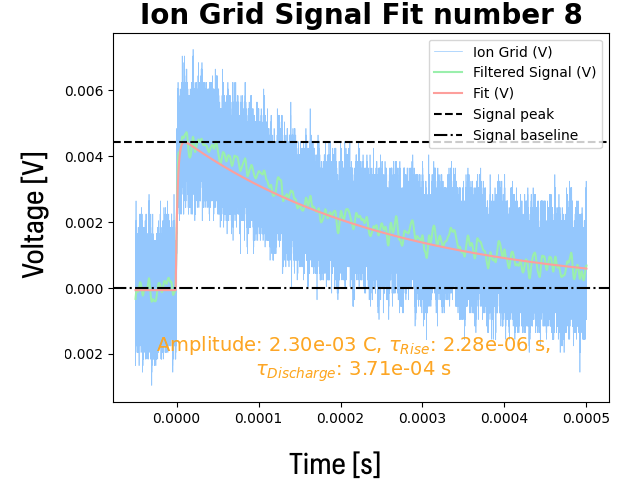
\includegraphics[width=6.5 in]{images/TargetSignal.png}
    \caption{An example fit to the target signal. The original signal is blue, the filtered signal is given in green and the fit is the red curve. The fit parameters are displayed in orange text.}
    \label{fig:targetfit}
\end{figure}

Prior to performing the target signal fit, the two gain stages (target low gain, target high gain) have to be combined into one signal. This is done by subtracting an average of the first 10 points from both signals to correct for the offsets in [dN]. Then, the low- and high-gain target signals are scaled by their respective pC/dN conversion values, given in \autoref{table:dntopc}. An example result where the target high gain channel saturates and is shown in \autoref{fig:combinedtarget}.

\begin{figure}[H]
    \centering
    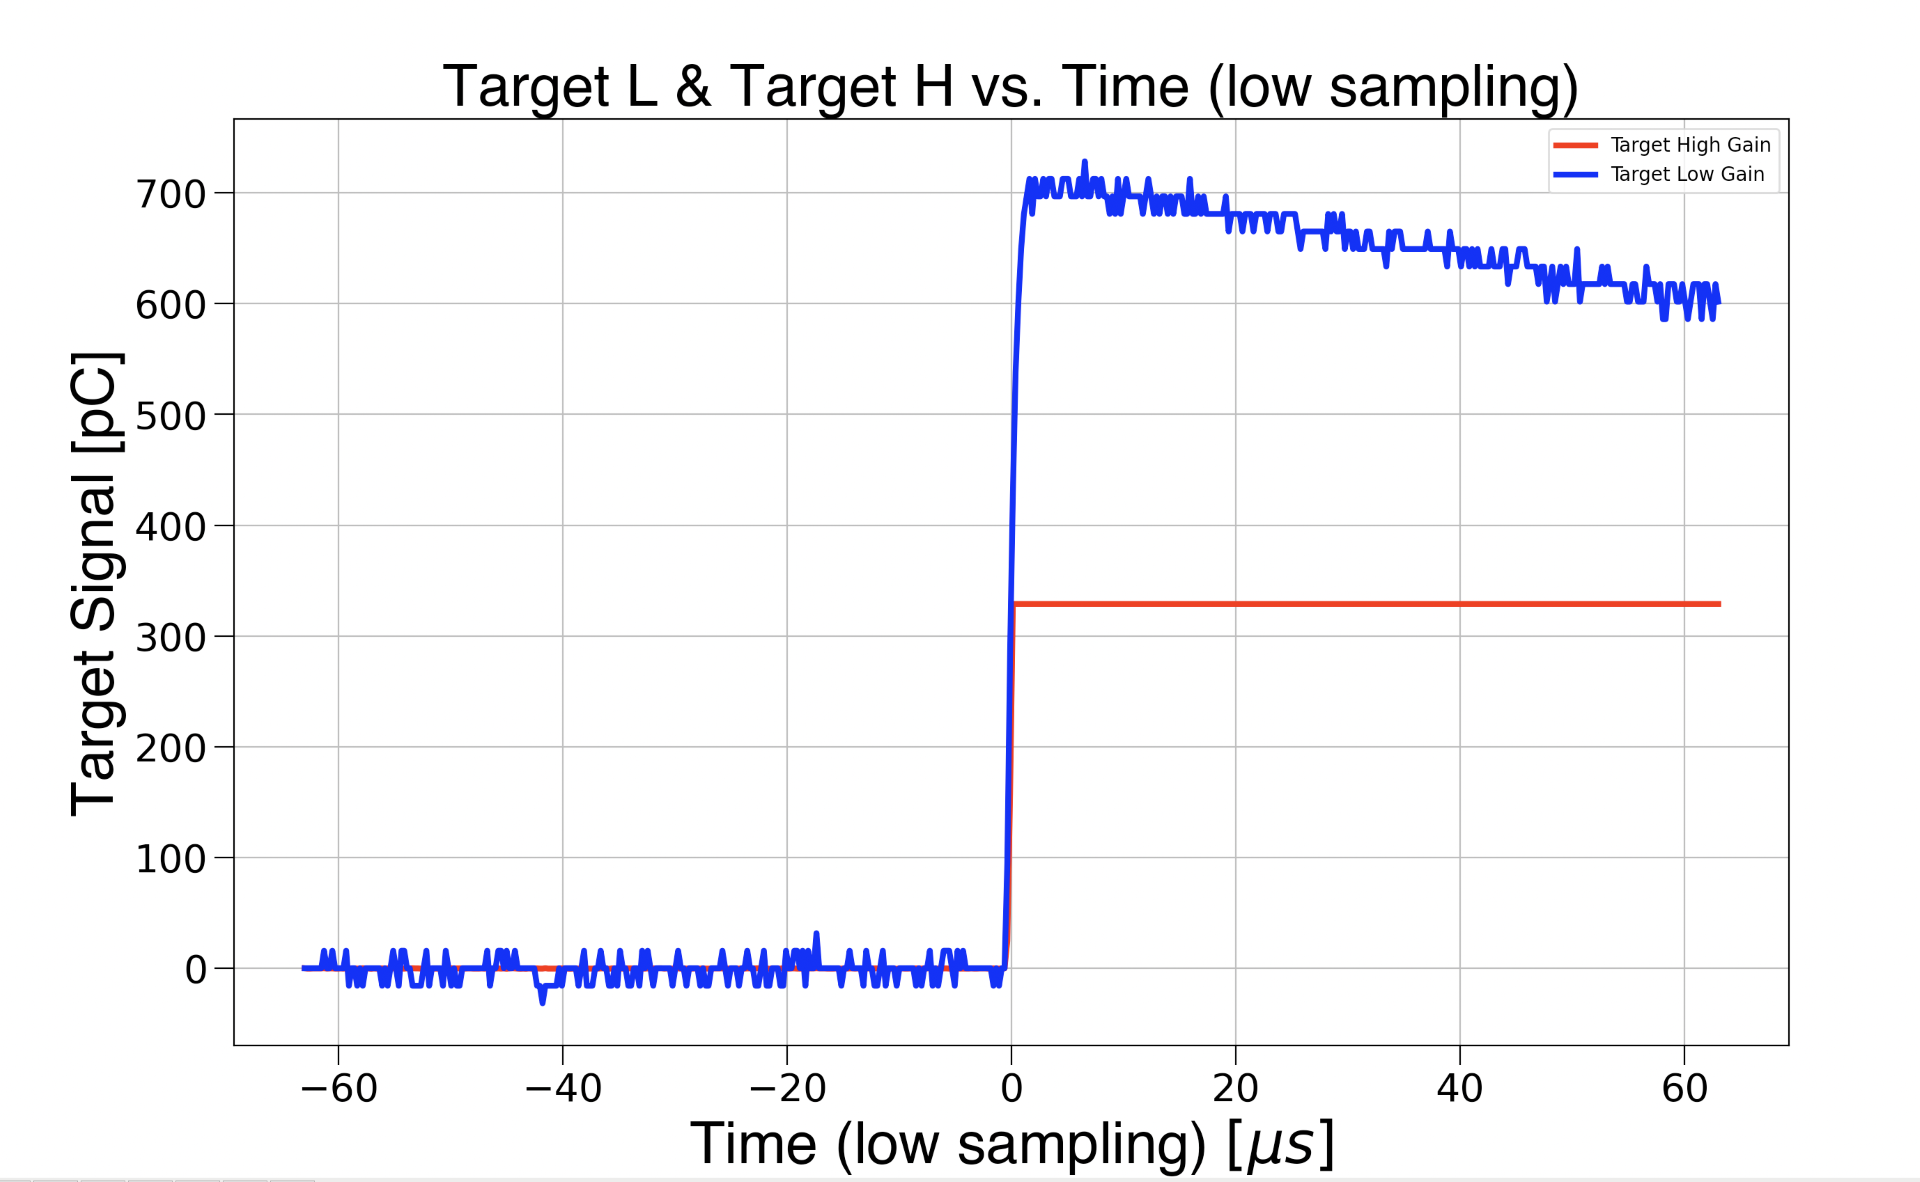
\includegraphics[width=6.5 in]{images/combined_target_signals.png}
    \caption{An example of combined target signals from Aluminum (Al) dust testing on the IDEX FM with the FM CSAs.}
    \label{fig:combinedtarget}
\end{figure}
Here, the target low gain (blue) is considered, as the high gain (red) saturates at 328.8 pC. The pC values \textbf{(in the specific case of the flight model with the flight CSAs)} were obtained from \autoref{table:dntopc} and are .163 and 15.8357 [pC/dN] for the high and low gain channels, respectively. 

Designate the best waveform (single or combined) with a flag for how it was created ("fit data"). Put this in a flag that can represent any permutation.

The dust mass can be estimated from the numerical integral of the combined TOF spectrum and signal fits to combined target and ion grid channels. The dust particle's impact charge is proportional to both its mass and velocity (Collette, 2014). It is estimated by the amplitude of both the target and ion grid signals, and by the integral of the TOF spectrum. The total charge (\(Q_i\)) generated during a dust impact of mass \(m\), at velocity \(v\)) follows the power law
\begin{equation}
Q_{i} \propto m^{\alpha} v^{\beta},
\end{equation}
where the exponents \(\alpha\) and \(\beta\) vary with the composition of the target and projectile and are experimentally derived. Typical values for $\alpha$
 and $\beta$ fall between 1-2 and 2-5, respectively. 

 \begin{equation}
Y(v; A, a_1, a_2, a_3, v_b, v_c, k) = A\cdot v^{a_1}\left [ \left(1+(\frac{v}{v_b})^k\right)^{\frac{a_2 - a_1}{k}} \cdot \left(1+(\frac{v}{v_c})^k\right)^{\frac{a_3 - a_2}{k}}  \right],  
  \label{eq:cal}
\end{equation}

During calibration at the dust accelerator, the impact charge as measured by the amplitude of the target signal was compared to the mass and velocity reported by the accelerator metadata.

\begin{figure}
    \centering
    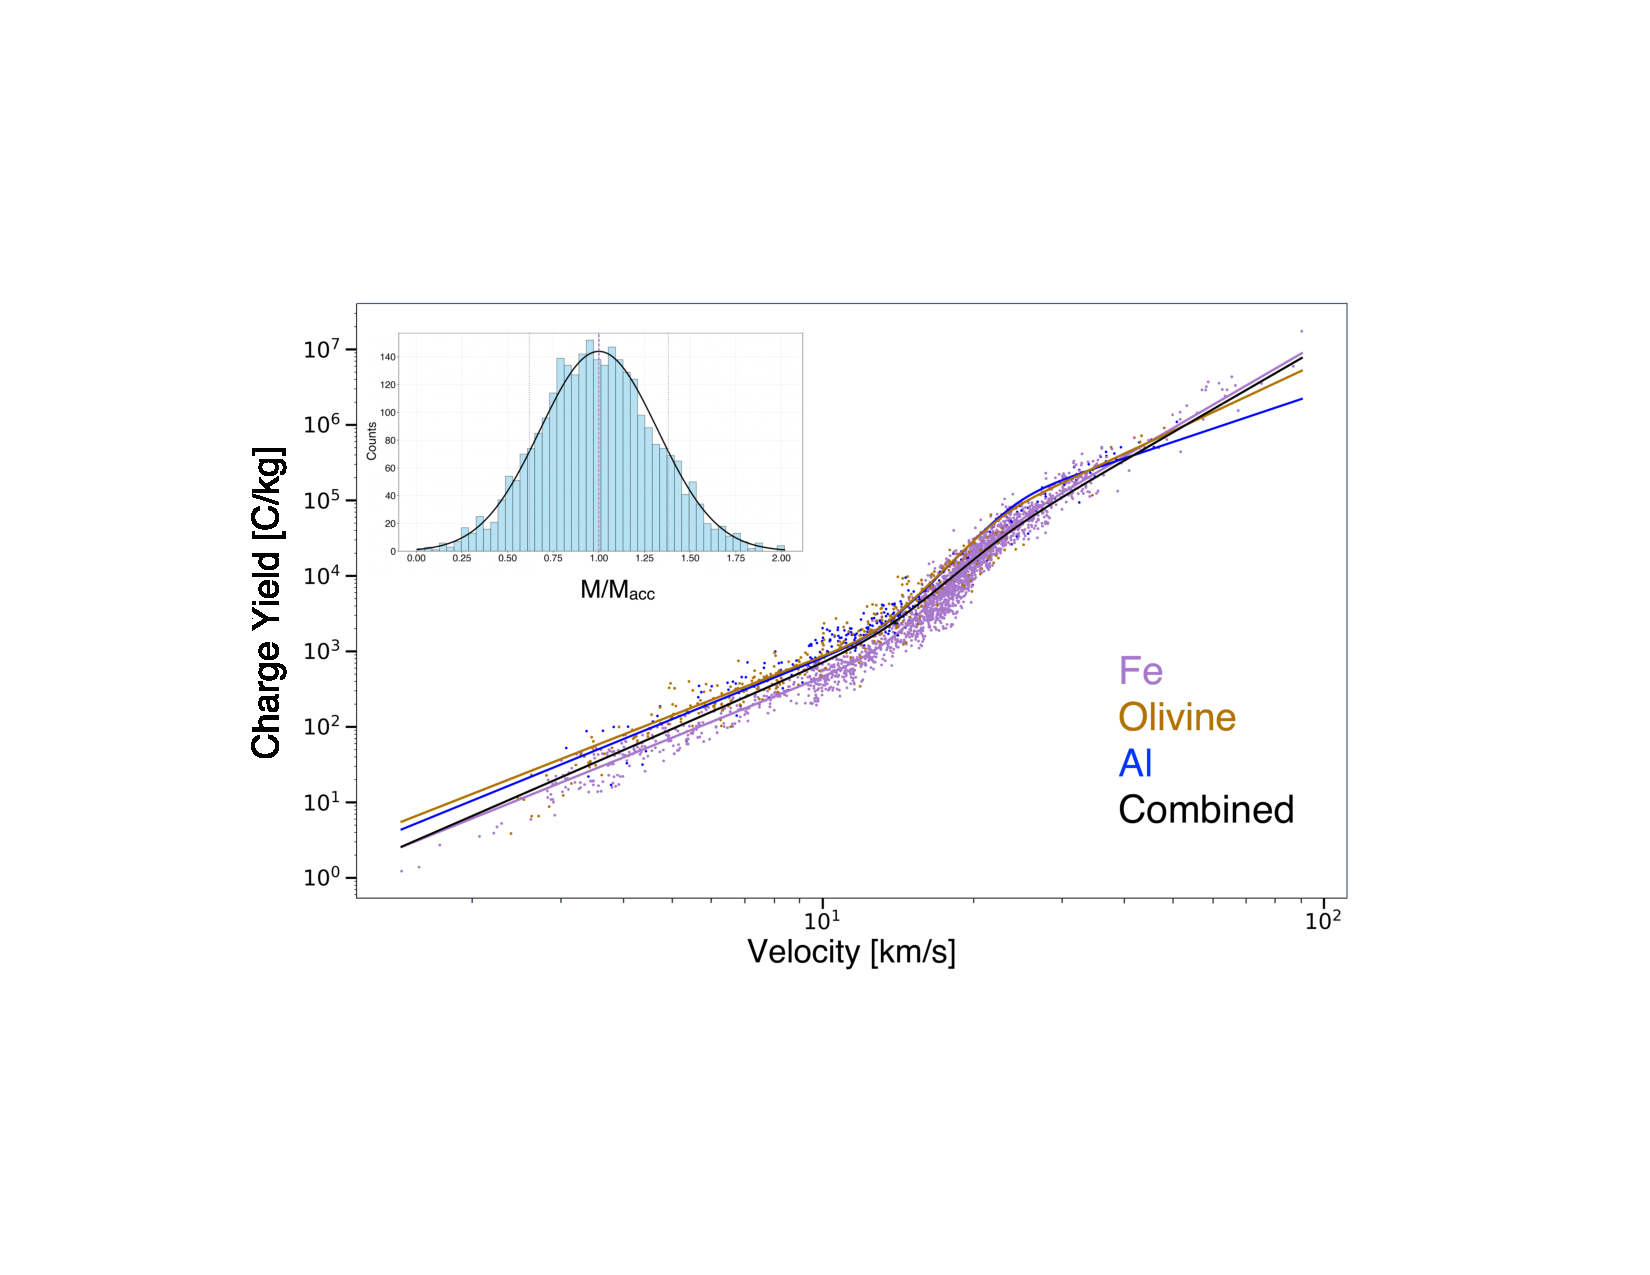
\includegraphics[width=\linewidth]{images/Ethan_yield.pdf}
    \caption{Charge yield for iron (red), aluminum (blue), and olivine (green dots) dust particles.  The insert shows the distribution of the ratio of the dust particle's mass, as calculated from the fit (\autoref{eq:cal}) for all materials combined, over the mass reported by the accelerator.}
    \label{fig:yield}
\end{figure}

The fit parameters for each material used to calibrate IDEX are given below.

\begin{table}[h!]
    \centering
               \renewcommand{\arraystretch}{1}
    \begin{tabular}{|lccccccccc|}


 \rowcolor{darkGrey}    \textcolor{white}{\textbf{}} & \textcolor{white}{\textbf{}} & \textcolor{white}{\textbf{}} &\textcolor{white}{\textbf{}} & \textcolor{white}{\textbf{$QT/M$}} &\textcolor{white}{\textbf{}} & \textcolor{white}{\textbf{}} & \textcolor{white}{\textbf{}} & \textcolor{white}{\textbf{}}&\textcolor{white}{\textbf{}} \\
 \rowcolor{darkGrey}    \textcolor{white}{\textbf{Material}} & \textcolor{white}{{$A$}} & \textcolor{white}{{$a_1$}} &\textcolor{white}{{ $a_2$}} & \textcolor{white}{{$a_3$}} &\textcolor{white}{{$v_b$  [km/s]}} & \textcolor{white}{{$v_c$} [km/s]} & \textcolor{white}{{k}} & \textcolor{white}{{$\sigma$}}&\textcolor{white}{\textbf{$\Delta M_Y$}} \\
        Fe & -0.02 & 2.7 & 6.7 & 3.9 & 13.0 & 23.7 & 11.6& 0.35 & 1.41 \\
   Olivine & 0.32 & 2.6 & 6.7 & 3.1 & 13.0 & 22.8 & 13.9 &0.32 & 1.37 \\
   Al      &0.21  & 2.7 & 6.8 & 2.2 & 13.1 & 24.6 & 12.3 &0.43 & 1.51 \\
Combined   & 0.06 & 2.8  & 5.9 & 4.1 & 13.0 & 22.7  & \ 8.2& 0.40 &1.47\\
     \hline
 \rowcolor{darkGrey}    \textcolor{white}{\textbf{}} & \textcolor{white}{\textbf{}} & \textcolor{white}{\textbf{}} & \textcolor{white}{\textbf{}} & \textcolor{white}{\textbf{{$v$}}} & 
 \textcolor{white}{\textbf{}} & \textcolor{white}{\textbf{}}  & \textcolor{white}{\textbf{}} & \textcolor{white}{\textbf{}}& \textcolor{white}{\textbf{}} \\
  \rowcolor{darkGrey}    \textcolor{white}{\textbf{Material}} & \textcolor{white}{{$A$}} & \textcolor{white}{{$a_1$}} &\textcolor{white}{{ $a_2$}} & \textcolor{white}{{$a_3$}} &\textcolor{white}{{$QT_{\tau}^b$  [$\mu$s]}} & \textcolor{white}{{$QT_{\tau}^c$} [$\mu$s]} & \textcolor{white}{{k}} & \textcolor{white}{\textbf{$\sigma$}}&\textcolor{white}{\textbf{$\Delta v_{QT}$}} \\
 Combined   & 3.6 & -0.2  & -2.0 & 0.38 &\  5.1 & 13.7  & 13.3 & 0.28 & 1.33 \\
     \hline
    \end{tabular}
    \caption{The parameters of the fit of the charge yield as function of the impact speed $Y(v; A, a_1, a_2, a_3, v_b, v_c, k)$ ($top$) and the impact speed as function of the target signal rise time $v(QT_{\tau}; A, a_1, a_2, a_3, v_b, v_c, k)$  ($bottom$) using the same form \autoref{eq:cal}, the standard error $\sigma$ of the Gaussian fitted to the ratio of the fit over the data, and the error factor of the fit  $\Delta M_Y
    \simeq exp(\sqrt{\ln(1 + \sigma^2})$.
    }
\label{tab:params}
\end{table}

In addition to our charge yield curve, our calibration campaign also consisted of developing trends for the target rise time and target to ion grid collection efficiency as a function of speed.

\begin{figure}[H]
    \centering
    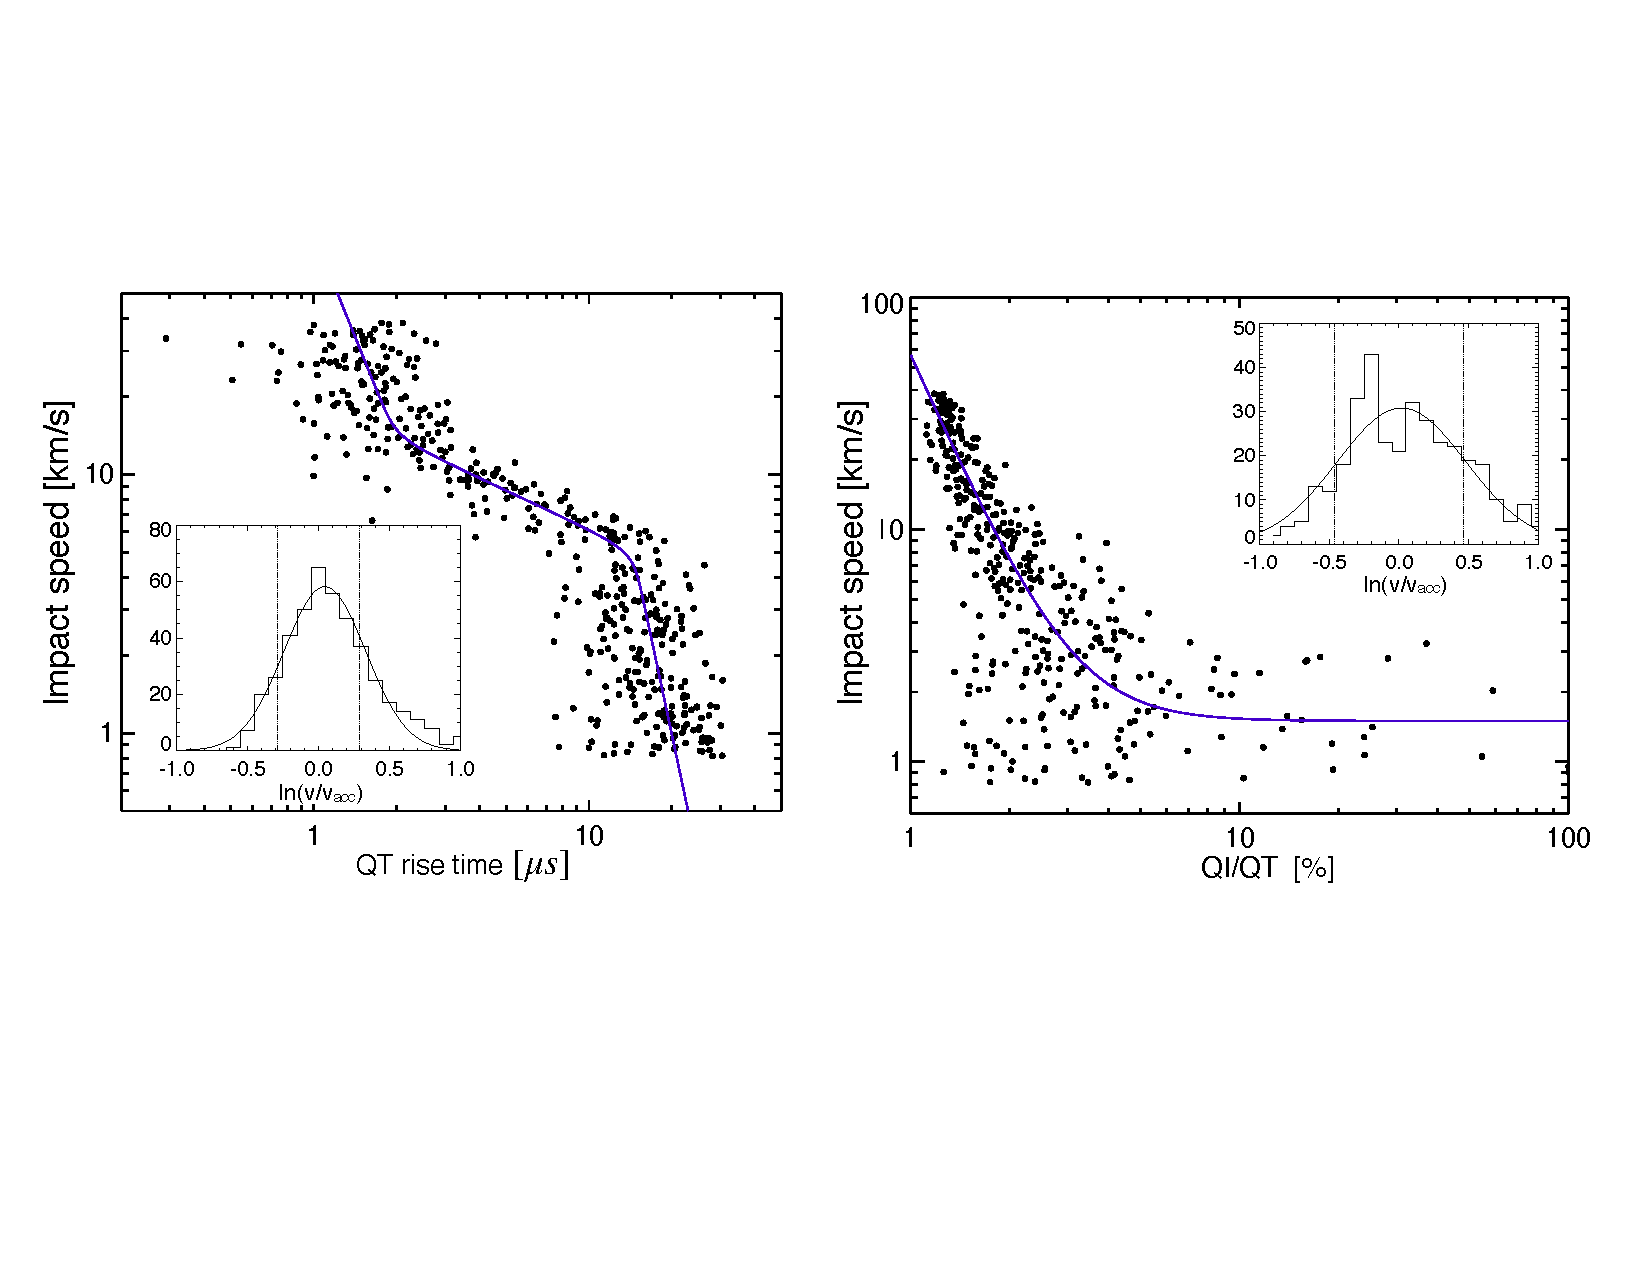
\includegraphics[width=6.5 in]{images/velocity_estimates.pdf}
    \caption{The impact speed of a dust particle as a function of the rise time of  $QT~ (left)$ and the ratio $QI/QT ~(right)$. The inserts show the Gaussian fits to the log of the ratios of the fit over the data, with $\sigma_{QT} \simeq 0.28$ and $\sigma_{QI/QT}  \simeq 0.46$, the error factors ($e^{\sigma}$) are $\Delta v_{QT} \simeq 1.33$  and $\Delta v_{QI/QT} \simeq 1.58$.}
    \label{fig:emtargetyield}
\end{figure}

This calibration curve is the result of both iron and aluminum dust impacts on the IDEX engineering model (EM) using the ground support equipment (GSE) CSAs. It is used at level 2A to provide an estimate for the dust mass with an error factor $\leq$ 2. 

In addition to fitting the target and ion grid signals for impact charge, the TOF mass spectrum's x-axis is converted from time to mass. The algorithm to do so is delineated as follows:

\begin{mdframed}[backgroundcolor=backcolour]{
\begin{enumerate}
    \item Make a vector with all zeros and a length of 8189, same as the TOF length of record: \( t_i \).
    \item Make a vector for masses \( m_i \): 1, 2, 3, 4, …, 200 (200 length, and the elements are the integers 1, 2, 3, …, 200).
    \item Calculate the 200 times (\( T_i \)-s) these masses should show up for a \( T_{\text{off}} = 0 \) and stretch \( A \) (best guess):
          \[
          T_i = T_{\text{off}} + A \sqrt{m_i}
          \]
          and set the closest \( t_i = 1 \) to each of the calculated \( T_i \)-s, leaving the rest as zero.
    \item Calculate the cross-correlation with the original TOF; the maximum will give you the best lag (\( T_{\text{off}} \)) for a given \( A \).
    \item Use an extrema finder to determine the best \( A \). 
\end{enumerate}
} \end{mdframed}

% Once the signal has been fitted, a linear equation is used to convert the amplitude of the fit from pC to V. This linear equation is derived from fits made to the CSAs during EM calibration. An example EM calibration fit is shown in figure~\ref{fig:csacal}.

% \begin{figure}[H]
%     \centering
%     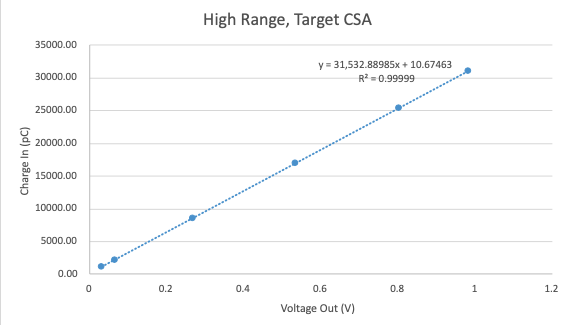
\includegraphics[width=\linewidth]{images/targetcsacal.png}
%     \caption{An example linear fit for the low gain (high range) target CSA.}
%     \label{fig:csacal}
% \end{figure}



\section{Level 2A to 2B Processing}
For the level 2B  data product, a spectrogram of the number of dust hits as a function of both mass and time will be generated. The simulation data depicted in \autoref{fig:isdpop} can be used to generate example files for these. The dataset records the count rate of detected dust particle impacts as a function of several key parameters: 


\begin{itemize}
    \item \textbf{Time of Impact} ($t$) - The timestamp of each dust detection event.
    \item \textbf{Spin Phase} ($\phi$) - The spacecraft spin phase at the time of detection. This is given in quadrants (0, 90, 180, 270).
    \item \textbf{Mass or Charge} ($m/q$) - The estimated mass or charge of the detected dust particle.
    \item \textbf{Count rate} ($N/\Delta t_{acc}$) - The number of detected dust particles in a given bin per accumulation time $t_{acc}$, where the accumulation time is the width of the time bin subtracted by any dead times.
\end{itemize}

\noindent\textbf{Science Acquisition Timestamp Extraction}

The Science Data Center (SDC) uses IDEX event telemetry to determine periods of science data collection. The IDEX instrument generates event files containing operational state information that are ingested and decommutated daily by the SDC.

The Level~2B (L2B) processing pipeline is triggered monthly and includes all event CDF files from the preceding month plus a two-week buffer period. This span ensures complete coverage for determining instrument operational states across processing boundaries.

The SDC processes event datasets through the following steps:
\begin{enumerate}
  \item \textbf{Data Preparation:} Event data are sorted chronologically by epoch timestamp, and duplicate entries are removed to ensure temporal consistency.

  \item \textbf{State Change Event Identification:} Science state-change events are identified by filtering for event packets with identifier \texttt{SCI\_STE} (Science State Event).

  \item \textbf{Parameter Reconstruction:} For each state-change event, two 16-bit parameter values are reconstructed by combining pairs of 8-bit telemetry parameters:
  \begin{itemize}
    \item \texttt{val1 = (el1par\_evtpkt << 8) | el2par\_evtpkt}
    \item \texttt{val2 = (el3par\_evtpkt << 8) | el4par\_evtpkt}
  \end{itemize}

  \item \textbf{Acquisition State Classification:} State transitions are classified based on parameter value combinations:
  \begin{itemize}
    \item \emph{Science Start:} \texttt{val1=ACQSETUP} and \texttt{val2=ACQ} indicate transition to active data acquisition.
    \item \emph{Science Stop:} \texttt{val1=ACQ} and \texttt{val2=CHILL} indicate transition to idle/standby state.
  \end{itemize}
\end{enumerate}

The charge and mass estimates are placed into 10 bins for the Level 2B IDEX data product. These bins and their ranges are given in table \ref{tab:charge_mass_bins}.

% Requires in preamble (once): \usepackage[table]{xcolor} \definecolor{darkGrey}{RGB}{77,77,77}

\begin{table}[h!]
\centering
\renewcommand{\arraystretch}{1.9}
\setlength{\tabcolsep}{8pt}
\begin{tabular}{|c|c|c|}
\hline
\rowcolor{darkGrey}
\textcolor{white}{\textbf{Bin}} &
\textcolor{white}{\textbf{Mass range [kg]}} &
\textcolor{white}{\textbf{Charge range [pC]}} \\
\hline
1  & $6.31\times10^{-17}$--$1.00\times10^{-16}$ & $1.00\times10^{-1}$--$3.16\times10^{-1}$ \\
2  & $1.00\times10^{-16}$--$1.58\times10^{-16}$ & $3.16\times10^{-1}$--$1.00\times10^{0}$ \\
3  & $1.58\times10^{-16}$--$2.51\times10^{-16}$ & $1.00\times10^{0}$--$3.16\times10^{0}$ \\
4  & $2.51\times10^{-16}$--$3.98\times10^{-16}$ & $3.16\times10^{0}$--$1.00\times10^{1}$ \\
5  & $3.98\times10^{-16}$--$6.31\times10^{-16}$ & $1.00\times10^{1}$--$3.16\times10^{1}$ \\
6  & $6.31\times10^{-16}$--$1.00\times10^{-15}$ & $3.16\times10^{1}$--$1.00\times10^{2}$ \\
7  & $1.00\times10^{-15}$--$1.58\times10^{-15}$ & $1.00\times10^{2}$--$3.16\times10^{2}$ \\
8  & $1.58\times10^{-15}$--$2.51\times10^{-15}$ & $3.16\times10^{2}$--$1.00\times10^{3}$ \\
9  & $2.51\times10^{-15}$--$3.98\times10^{-15}$ & $1.00\times10^{3}$--$3.16\times10^{3}$ \\
10 & $3.98\times10^{-15}$--$1.00\times10^{-14}$ & $3.16\times10^{3}$--$1.00\times10^{4}$ \\
\hline
\end{tabular}
\caption{Bin definitions for mass and charge used for IDEX L2B data products.}
\label{tab:charge_mass_bins}
\end{table}

For the edge case that a mass or charge value is below the value 

The following table presents a sample of the Level 2B data product. The values represent binned counts of detected dust particles:






\begin{table}[h]
    \centering
    \caption{\textbf{Daily Binned Dust Hit Counts as a Function of Time, Spin Phase, and Mass/Charge}}
    \label{tab:dust_counts}
    \renewcommand{\arraystretch}{1.3}
    \setlength{\arrayrulewidth}{1.2pt}
    \begin{tabular}{c c c c}
        \hline\hline
        \textbf{Date (UTC)} & \textbf{Spin Phase (deg)} & \textbf{Mass/Charge ($\si{kg}$ or $\si{C}$)} & \textbf{Rate ($s^{-1}$)} \\
        \hline\hline
        2027-02-18 & \textbf{0}  & \textbf{$1.2 \times 10^{-15}$}  & \textbf{32}  \\
        2027-02-19 & \textbf{90} & \textbf{$3.5 \times 10^{-16}$}  & \textbf{60} \\
        2027-02-20 & \textbf{180} & \textbf{$2.51 \times 10^{-15}$}  & \textbf{25}  \\
        2027-02-21 & \textbf{270} & \textbf{$4.8 \times 10^{-16}$}  & \textbf{48} \\
        \hline\hline
    \end{tabular}
\end{table}

\textbf{Please note that: }
\begin{itemize}
    \item Times are given in Coordinated Universal Time (UTC).
    \item Spin phase is defined relative to an inertial (despun) reference frame.
    \item Mass and charge values are estimated using calibration data.
\end{itemize}

\section{Level 2A to 2C Processing}

Generate pointing sets from level 2A. All events will be dust, so pointing sets follow directly. Count rates are encoded in the pointing sets. We want RTN for IDPs, EJ2000 for ISD. A time-ordered list of time, boresight vector for every impact. We will also need accumulation times. Disregard events that are flagged as SW triggers.

For the level 2C data products, maps of flux, rates and composition will be generated, using the IBEX ENA maps as reference. An example of a historical dust map for the interstellar dust is shown in \autoref{fig:isdmap}.


\begin{figure}[H]
    \centering
    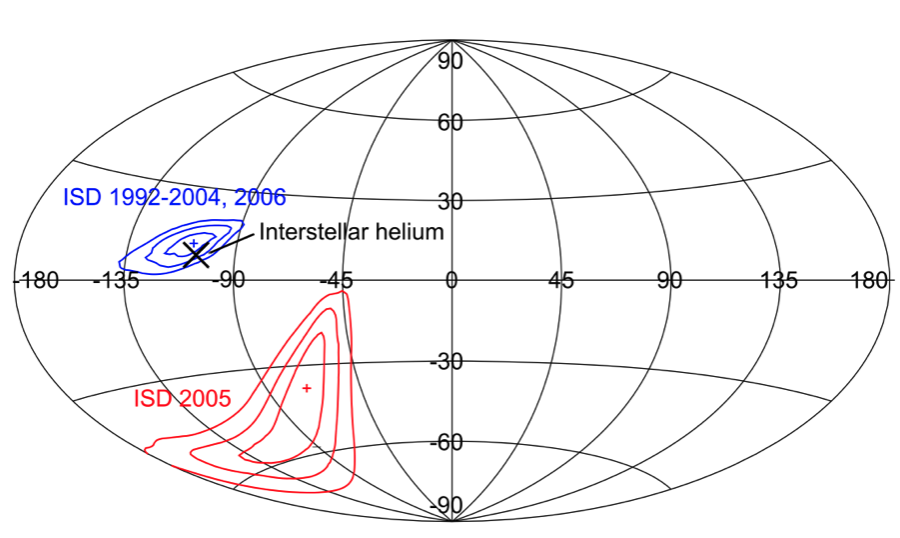
\includegraphics[width=6.5 in]{images/isd_deflection_map.png}
    \caption{Map of the two different deflections of interstellar dust measured by Cassini's CDA and Ulysses from the nominal interstellar helium flow direction into the solar system. }
    \label{fig:isdmap}
\end{figure}.

These maps will require defining \textbf{pointing sets}, which contain the data binned by instrument boresight vector. For IDEX maps, each dust impact is assumed to come directly from the boresight direction (neglecting the 50-degree field-of-view).

Typical data for a 2 year mission are shown in figure \ref{fig:mappedcounts}. The y and x axes represent the EJ2000 latitude and longitude, respectively. The incoming ISD direction is apparent from the enhancement at (8, -118).

\begin{figure}[h!]
    \centering
    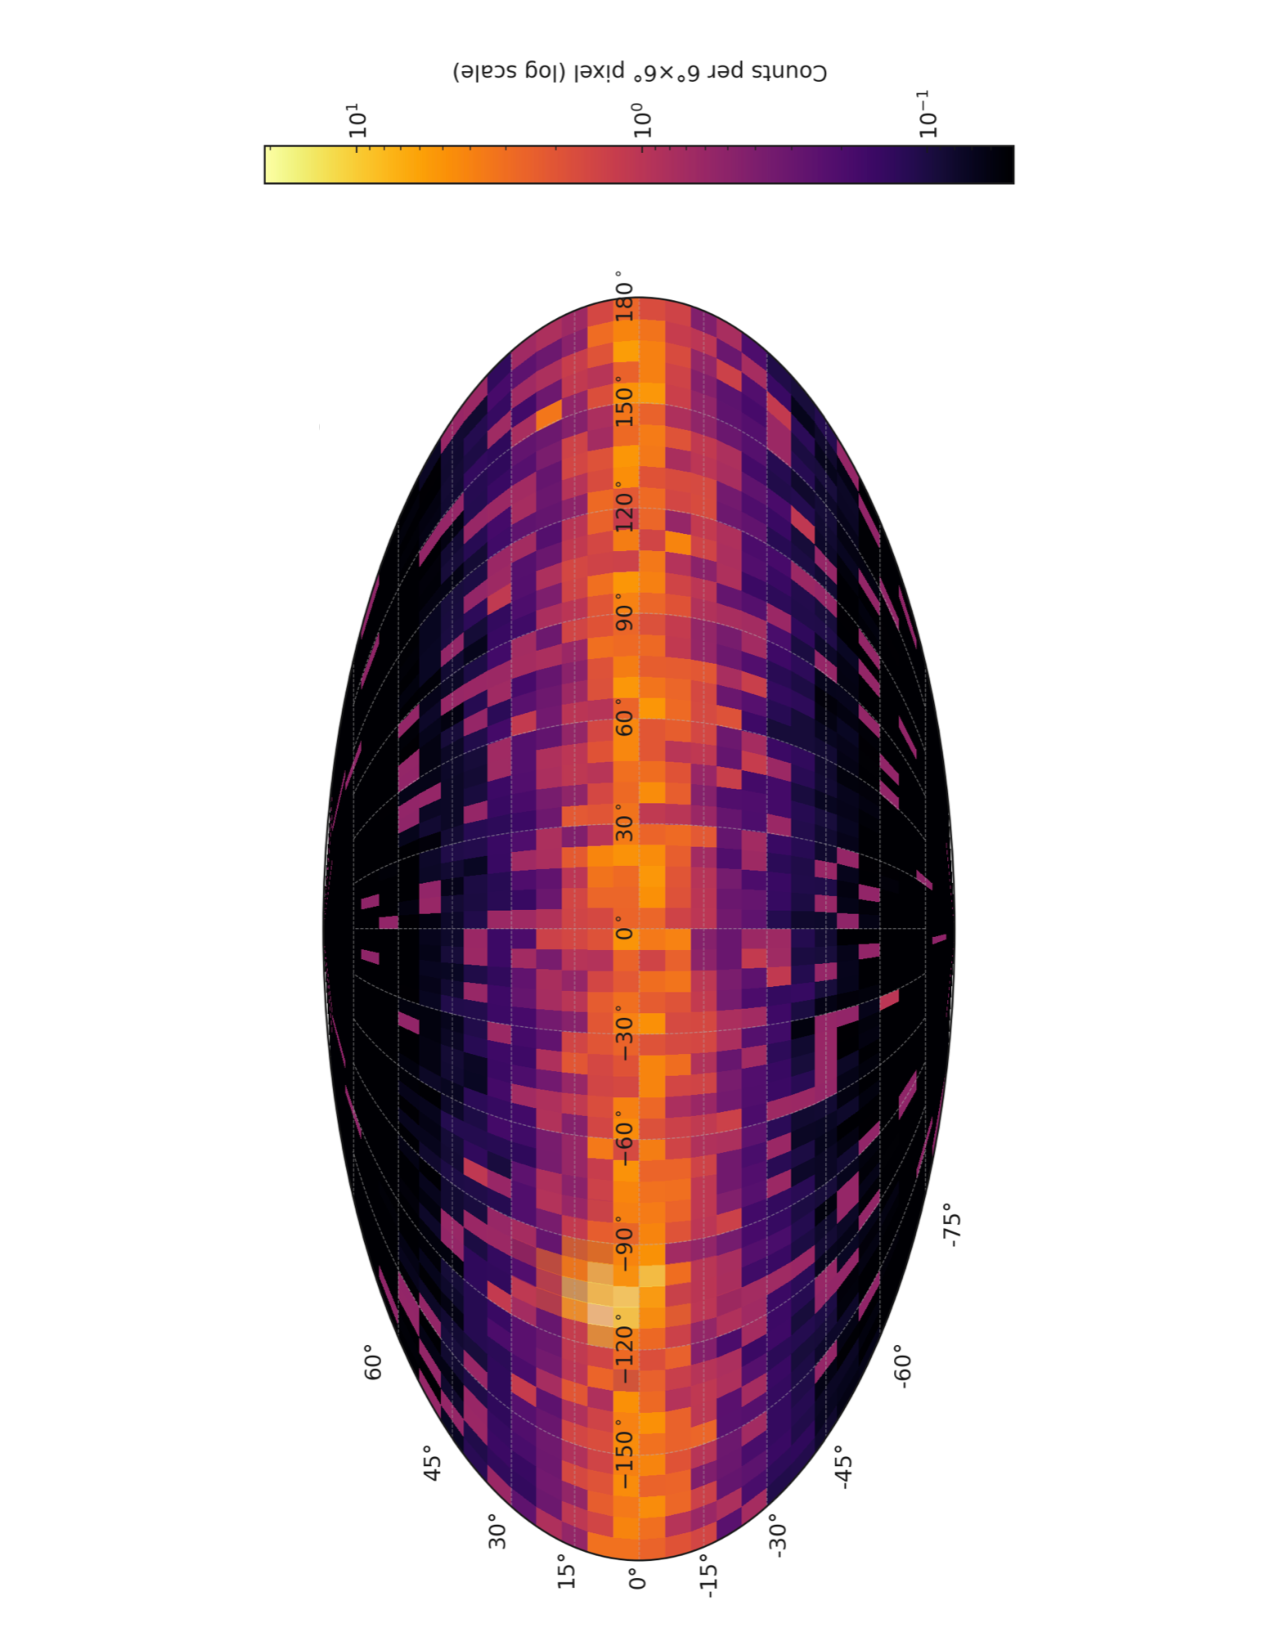
\includegraphics[angle=270, width=0.8\linewidth]{images/Mollweide_Zodiacal_dust_sky_map.pdf}
    \caption{Total dust counts per 6 x 6 degree pixels in latitude and longitude in EJ2000. This is assuming a dust instrument mounted to a spacecraft at 1 AU, such as IDEX. These maps will be used for direct comparison of the COMIT model's results with IMAP results. In addition to total dust counts, they will be generated for a given impact charge, mass and dust composition type (silicate, organic, etc.) for further comparison with IDEX.}
    \label{fig:mappedcounts}
\end{figure}
